\section{Problem 1}

\subsection{Question}
\vspace*{10pt}
Determine if the friendship paradox holds for your Twitter account.
Since Twitter is a directed graph, use \enquote{followers} as value you measure 
$($i.e., \enquote{do your followers have more followers than you?}$)$.\\
\\
Generate the same graph as in question \#1, and calcuate the same 
mean, standard deviation, and median values.\\
\\
For the Twitter 1.1 API to help gather this data, see:
\\
\url{https://dev.twitter.com/docs/api/1.1/get/followers/list}
\\
If you do not have followers on Twitter (or don't have more than 50),
then use my twitter account \enquote{phonedude\_mln}.

\subsection{Answer}
\vspace{2mm}
A Python program, {\it qet\_graphml.py}, has been written to extract\cite{xml} number of friends that Dr. Nelson friends have. The program will search for this information in a file called {\it mln.graphml} \cite{graphML}. The output of this program would be like the following:
\vspace{5mm}

\begin{figure}[h!]
\centering
\fbox{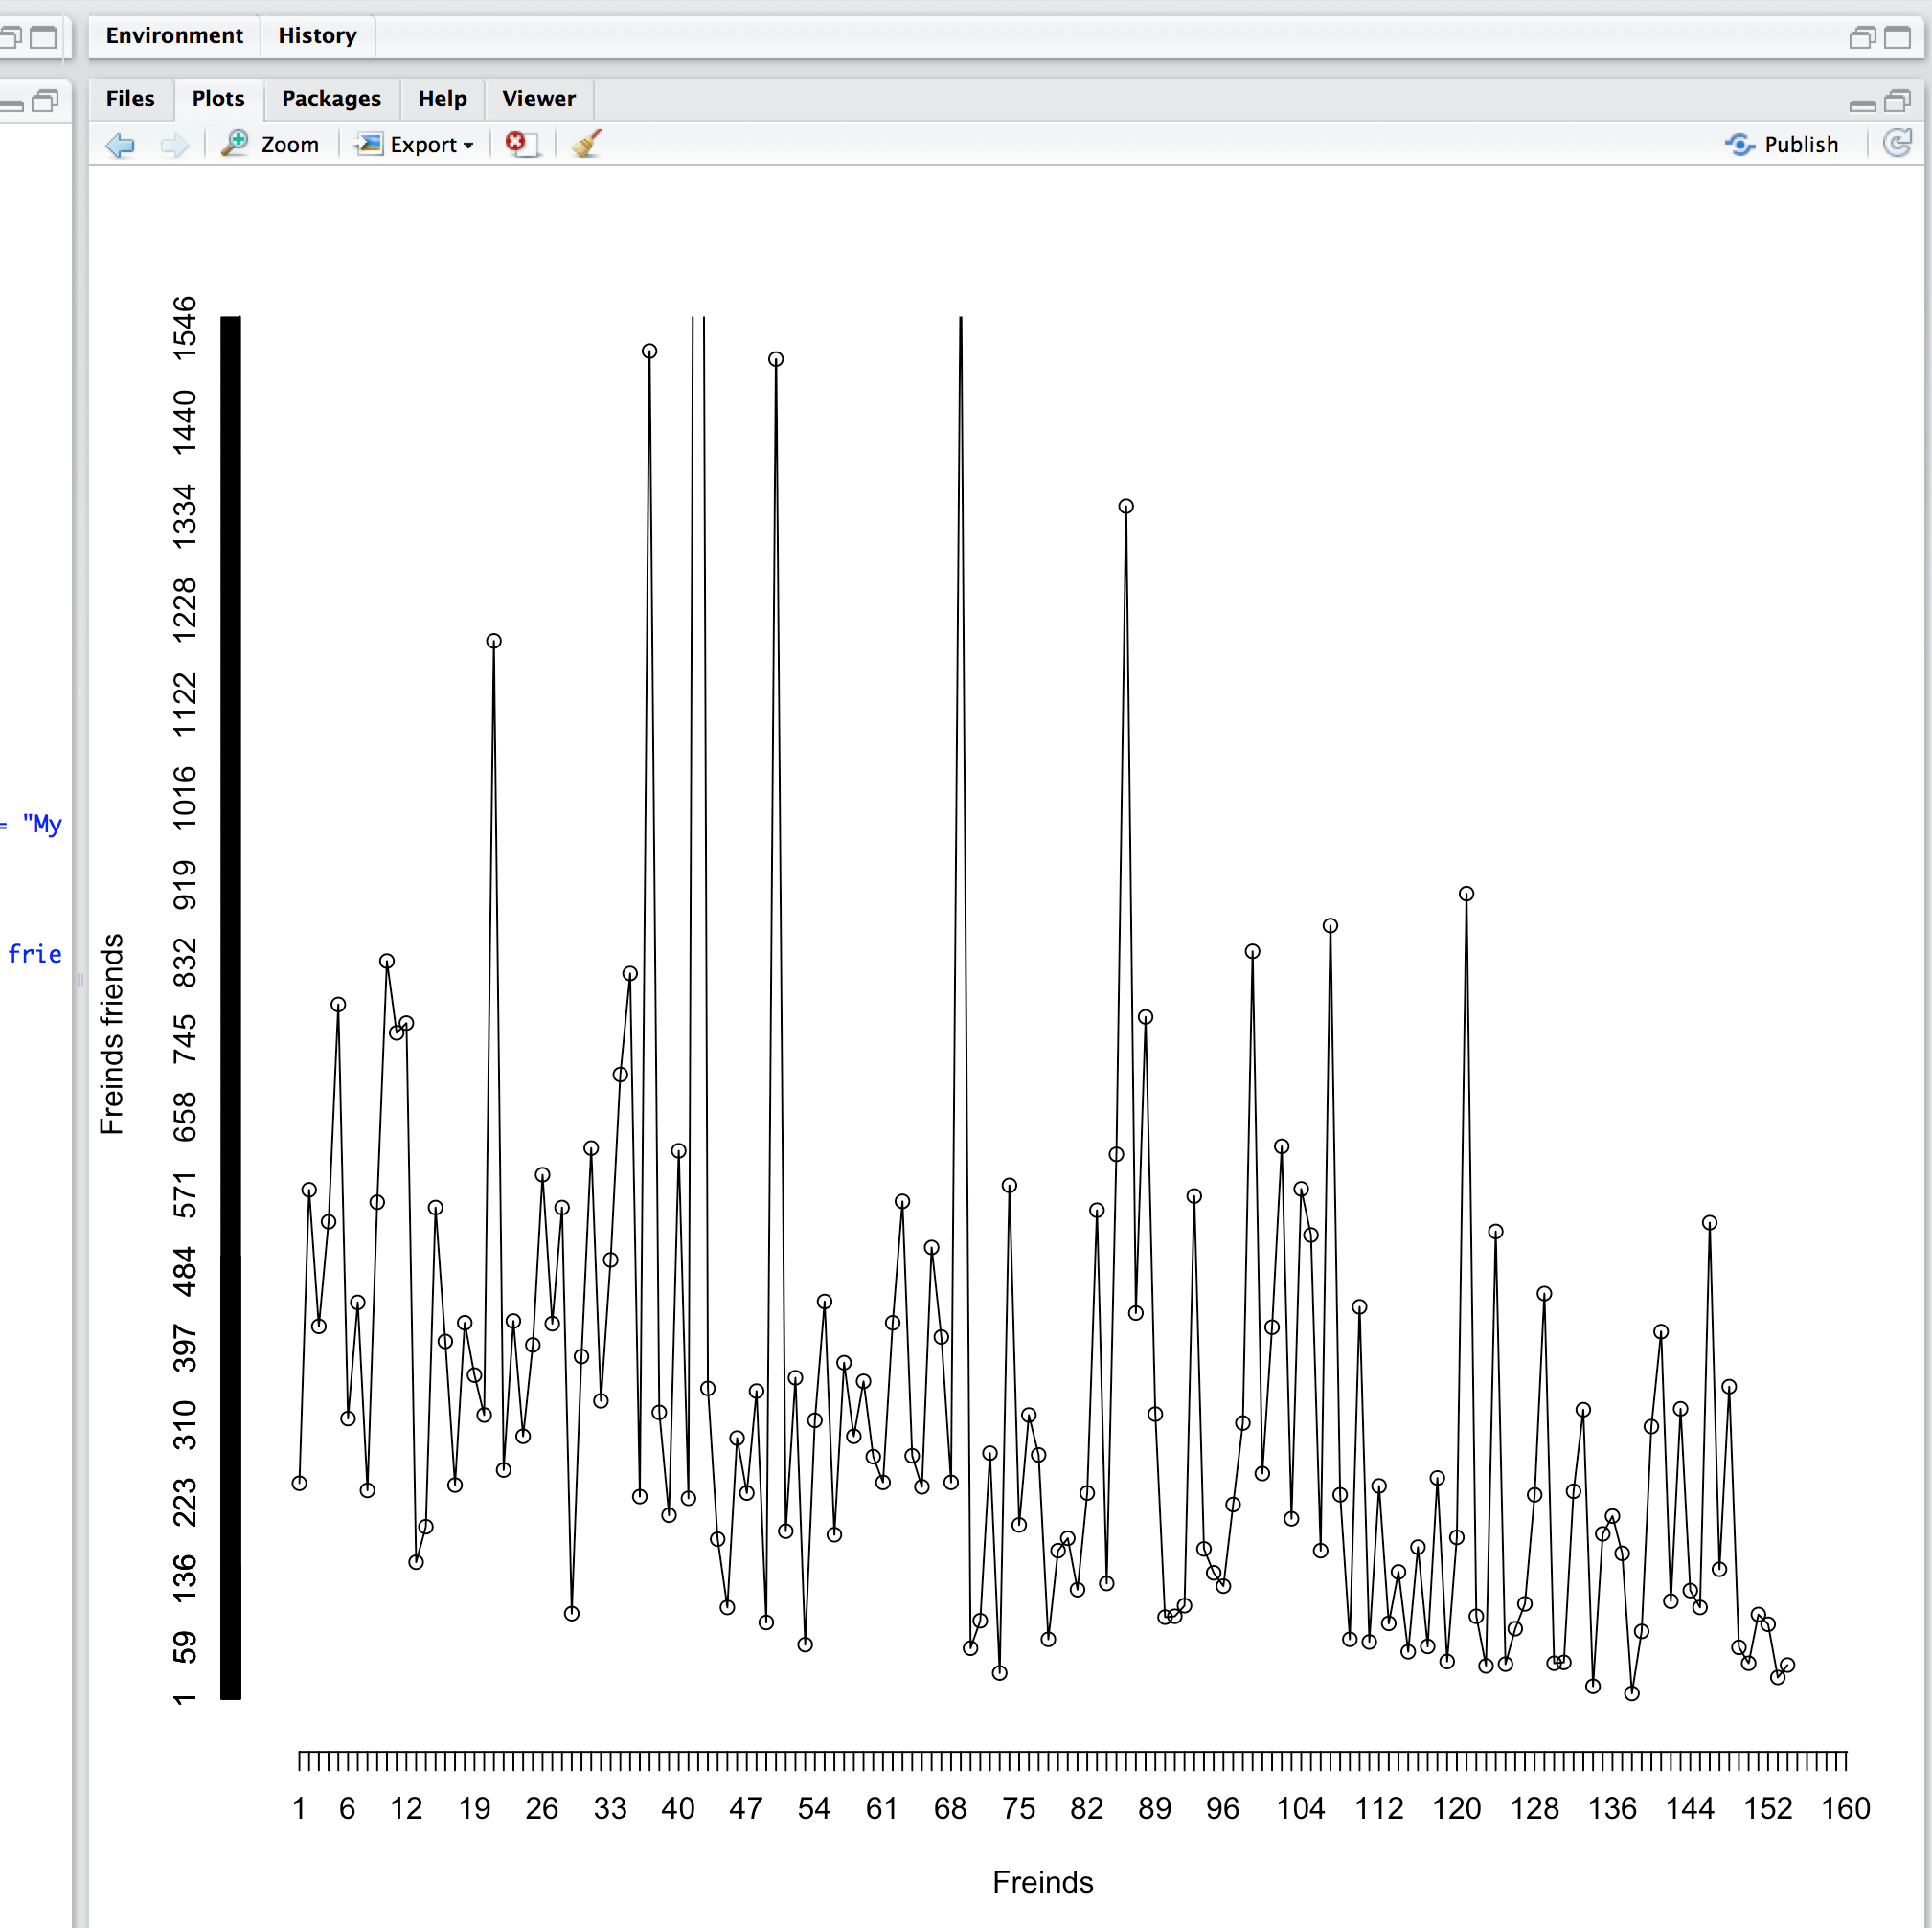
\includegraphics[scale=0.75]{q1/fig1.png}}
\caption{Sample output of number of friends}
\label{fig:number_friends_1}
\end{figure}
\vspace*{5pt}

\begin{figure}[h!]
\centering
\fbox{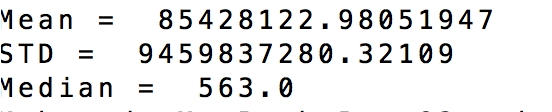
\includegraphics[scale=0.85]{q1/fig2.png}}
\caption{Sample output of number of friends}
\label{fig:number_friends_2}
\end{figure}
\clearpage
\newpage
\vspace*{5pt}
\lstinputlisting[language=Python, caption={get\_graphml.py}, label=listing:graphml]{q1/get_graphml.py}

\vspace*{5pt}

I would like to let you know that even though Dr. Nelson have 319 friends, only 165 allow me to see their number of friends. This will affect the statistical result. For example, instead of dividing by 319 to get the mean, we divide by 165.

The {\tt graphml\_counts} file was ordered in place with the Unix command in Listing \ref{listing:sort}. 
\\
\begin{lstlisting}[language=Bash,caption={Sort command},label=listing:sort]
Naina Sai Tipparti@DESKTOP-2FU7AJC ~/a4/q1 cat graphml_counts | sort -g -o graphml_counts
\end{lstlisting}

This file was then processed by the R script\cite{rscript} shown in Listing \ref{listing:R_graphml} to produce the graph in Figure \ref{fig:facebook_graphml}

\lstinputlisting[language=R, caption={Graph Creation Script for Facebook}, label=listing:R_graphml]{q1/plot_graphml.R}
\vspace{5mm}
\begin{figure}[h!]
\centering
\fbox{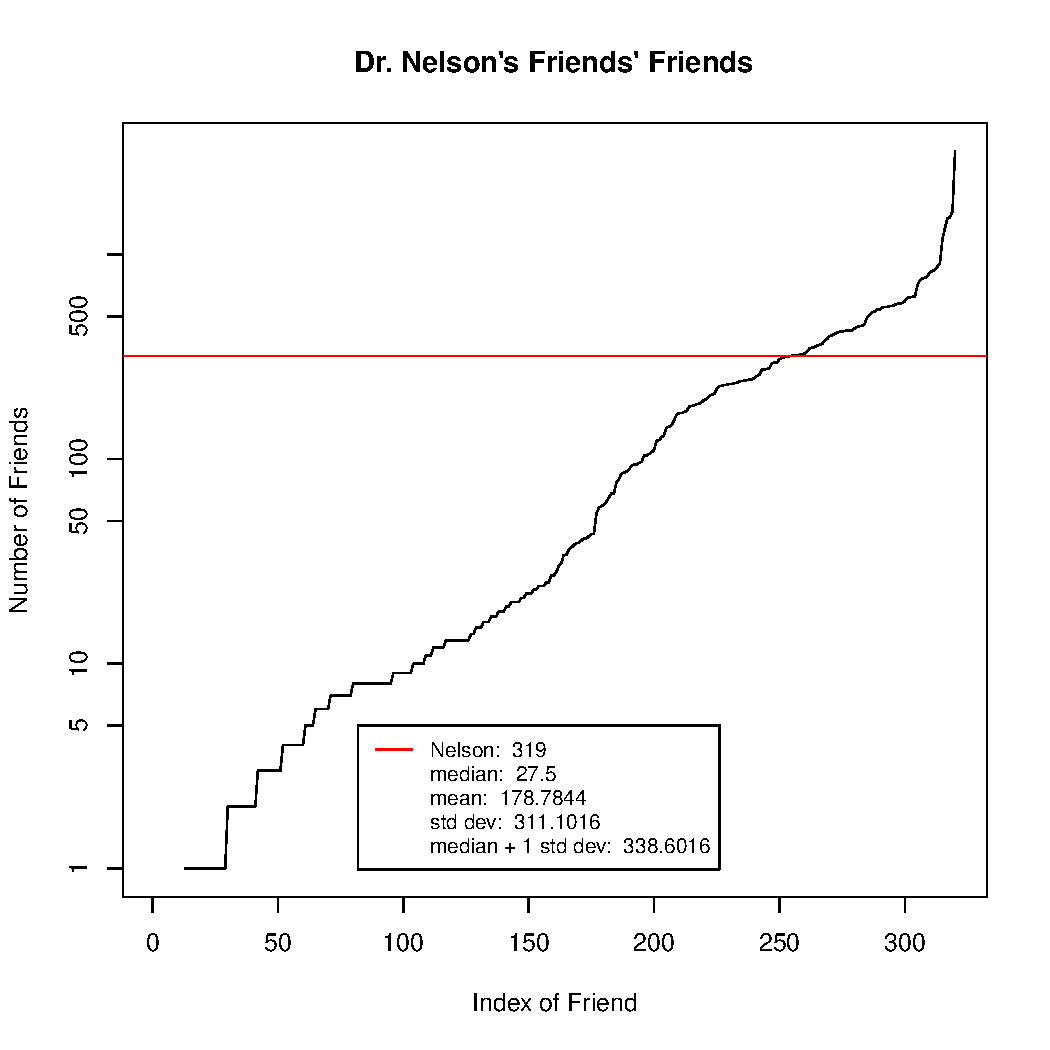
\includegraphics[scale=0.65]{q1/facebook_graphml.pdf}}
\caption{The Friendship Graph for Facebook}
\label{fig:facebook_graphml}
\end{figure}
\newpage
The median, mean and standard deviation were all calculated, with the median, mean and median plus one standard deviation.
\vspace*{2mm}
\begin{table}
\centering
\begin{tabular}{ l l }
\hline
\textbf{Mean} & 178.7844 \\
\textbf{Median} & 27.5 \\
\textbf{Std Dev} & 311.1016\\
\hline
\end{tabular}
\caption{Statistics on the count of Dr. Nelson Facebook Friends' Friends, values straight from R}
\label{tab:q1stats}
\end{table}

